\documentclass[twoside,10pt]{article}
\usepackage{amsmath,amsfonts,amsthm,fullpage}
\usepackage{algorithm}
\usepackage{algorithmic}
\usepackage{graphicx}
\usepackage{subcaption}
\renewcommand{\qedsymbol}{\rule{0.7em}{0.7em}}


\begin{document}

\title{ISYE 6740, Summer 2020, Homework 2}
\author{Arjun Singh}
\date{\today}
\maketitle



\subsection*{1. Order of faces using ISOMAP (30 points)}

The objective of this question is to reproduce the ISOMAP algorithm results that we have seen discussed in lecture as an exercise. The file \textsf{isomap.mat} (or \textsf{isomap.dat}) contains 698 images, corresponding to different poses of the same face. Each image is given as a 64 $\times$ 64 luminosity map, hence represented as a vector in $\mathbb R^{4096}$. This vector is stored as a row in the file. [This is one of the datasets used in the original paper for ISOMAP, J.B. Tenenbaum, V. de Silva, and J.C. Langford, Science 290 (2000) 2319-2323.] In this question, you are expected to implement the ISOMAP algorithm by coding it up yourself.

\begin{enumerate} 
\item[(a)] (10 points) Choose the Euclidean distance between images (i.e., in this case a distance in $\mathbb R^{4096}$). Construct a similarity graph with vertices corresponding to the images, and tune the threshold $\epsilon$ so that each node has at least 100 neighbors (this approach corresponds to the so-called $\epsilon$-Isomap). Visualize the similarity graph (you can visualize the graph  using various graph visualization packages, and illustrate a few images corresponds to nodes at different parts of the graph; you can be a bit creative here).

\begin{itemize}
\item Answer:\\
Figure 1 displays the similarity graph using the 100 nearest neighbours. In general, the images seem to be randomly oriented.
\begin{figure}[h!]
\begin{center}
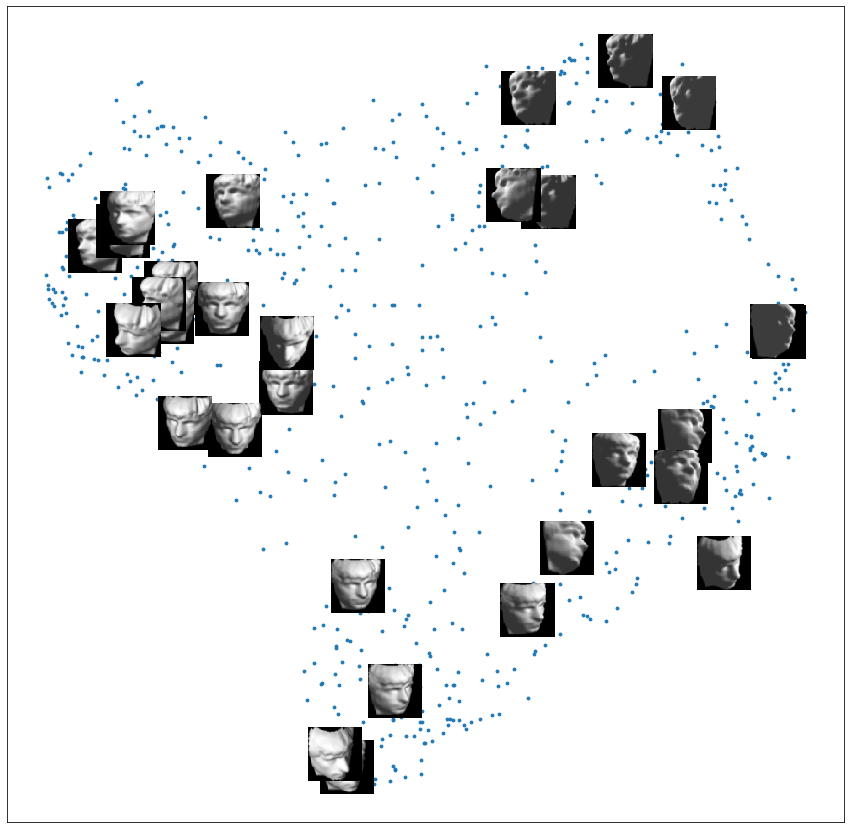
\includegraphics[totalheight=3in]{Images/Q1a.png}
\end{center}
\caption{Similarity graph with sample images}
\end{figure}
\end{itemize}
 
\item[(b)] (10 points) Implement the ISOMAP algorithm and apply it to this graph to obtain a $d$ = 2-dimensional embedding. Present a plot of this embedding. Find three points that are ``close'' to each other in the embedding space, and show what they look like. Do you see any visual similarity among them?

\begin{itemize}
\item Answer:\\
Figure 2 displays the embeddings and the corresponding images after performing the ISOMAP algorithm. We notice that after performing ISOMAP, the images are clustered within certain orientations. The bottom right of the plot is facing left whereas the left side of the plot is facing down and right. We also notice that the darker images are towards the top of the plot whereas the lighter images are at the bottom.
Although there is some structure to the output with similar head orientations grouped together, it is not completely well distributed as shown in the research paper.\\
After plotting 3 'close' points, as shown in Figure 3, we see that all selected images are facing the same direction.
\begin{figure*}[t!]
    \centering
    \begin{subfigure}[t]{0.5\textwidth}
        \centering
        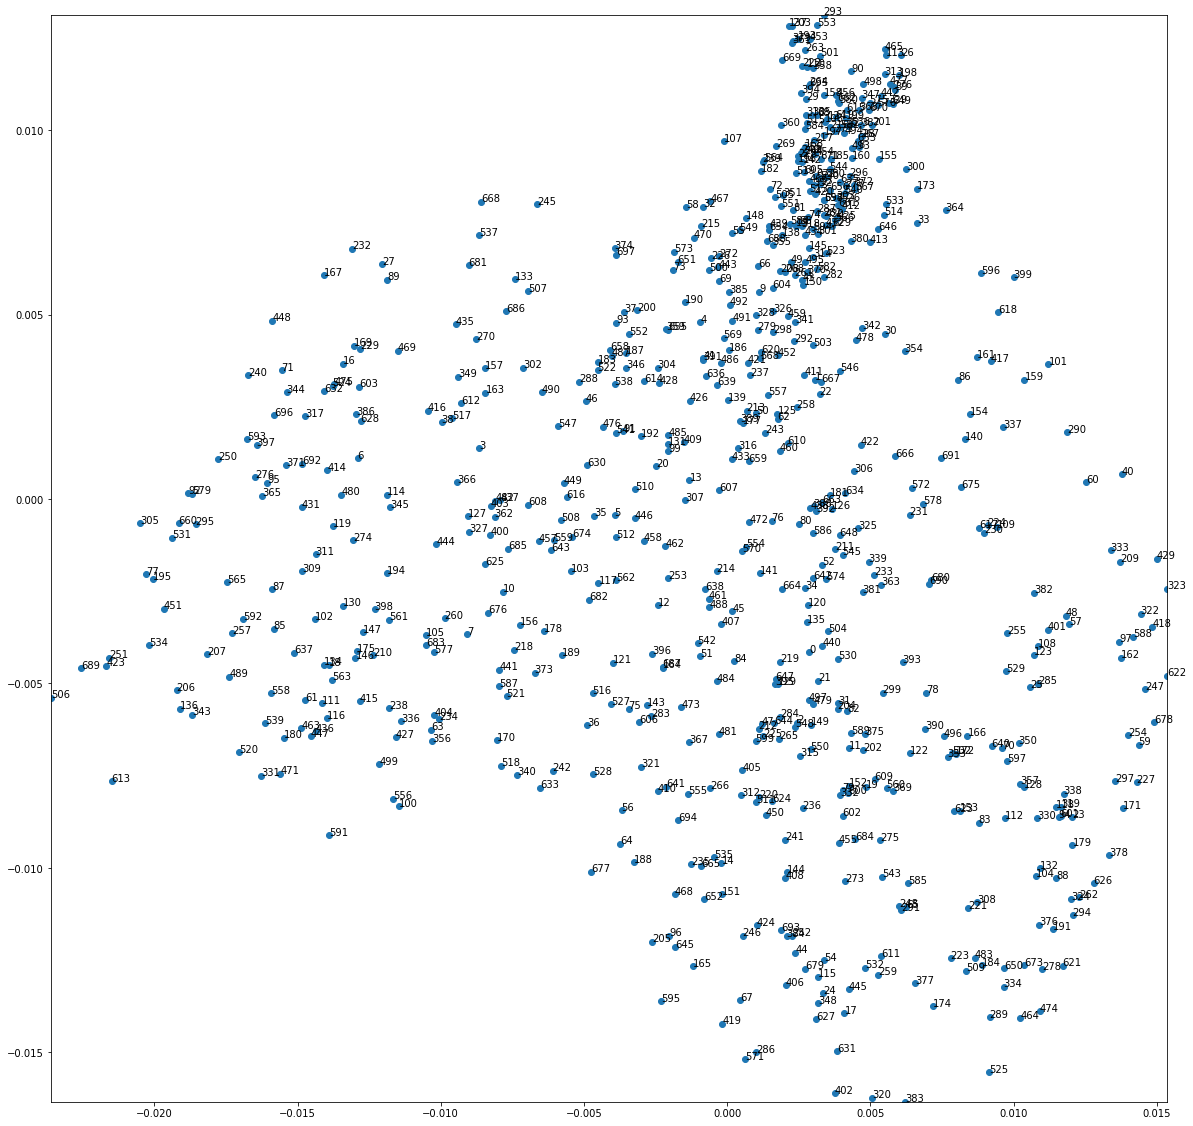
\includegraphics[height=3.1in]{Images/Q1bembeddings.png}
        \caption{2D Embedding}
    \end{subfigure}%
    ~ 
    \begin{subfigure}[t]{0.5\textwidth}
        \centering
        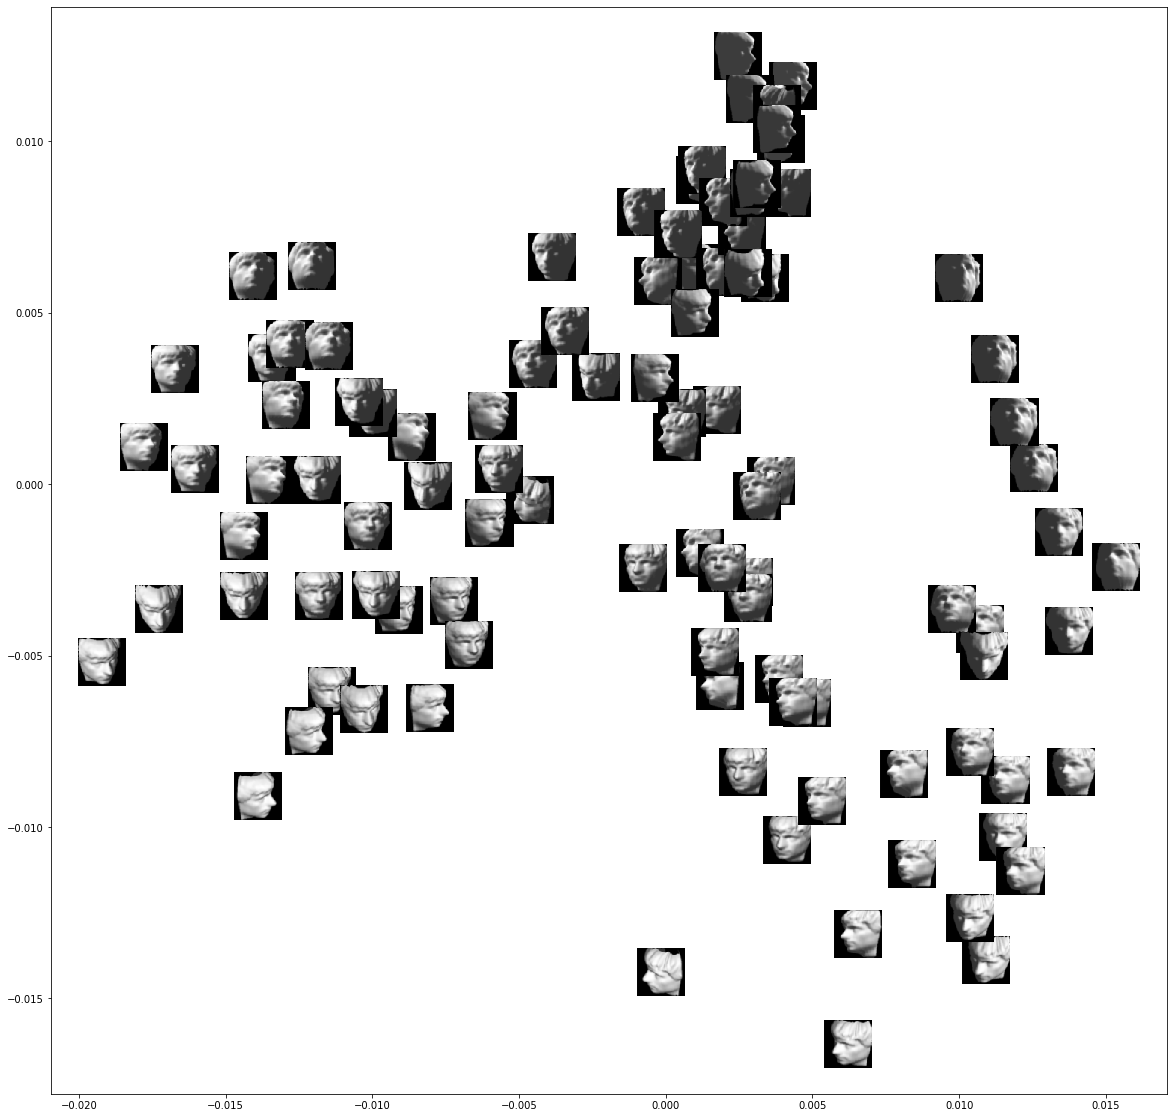
\includegraphics[height=3.1in]{Images/Q1bimages.png}
        \caption{Corresponding Images after ISOMAP}
    \end{subfigure}
    \caption{ISOMAP Algorithm Results}
\end{figure*}

\begin{figure}[h!]
\begin{center}
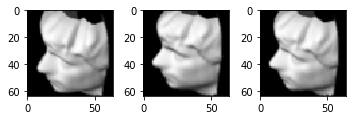
\includegraphics[totalheight=2in]{Images/Q1bsimilarity.png}
\end{center}
\caption{Visualizing 3 'close' points}
\end{figure}

\end{itemize}


\item[(c)] (10 points) Now choose $\ell_1$ distance (or Manhattan distance) between images (recall the definition from ``Clustering'' lecture)). Repeat the steps above. Again construct a similarity graph with vertices corresponding to the images, and tune the threshold $\epsilon$ so that each node has at least 100 neighbors. Implement the ISOMAP algorithm and apply it to this graph to obtain a $d$ = 2-dimensional embedding. Present a plot of this embedding.  Do you see any difference by choosing a different similarity measure, by comparing results in Part (a)(b) and Part (c)? 

\begin{itemize}
\item Answer:\\
Figure 4 displays the similarity graph using the Manhattan distance while Figure 5 shows the embeddings and the corresponding images. We notice that by using the Manhattan distances instead of the Euclidean distance, the images seem reversed. With the Manhattan distance, the lighter images are on  top whereas the darker images with shadows are on the bottom. The right side of the plot has an orientation of facing rightward and the left side has images facing leftward, which is opposite to the Euclidean distances plots seen above.
In general, images still seem to be clustered according the the orientation. After picking 3 close points, we observe that the algorithm still clusters similar images together, in this case choosing images that look up and slightly to the left. All 3 images also have a shadow on the right.

\begin{figure}[h!]
\begin{center}
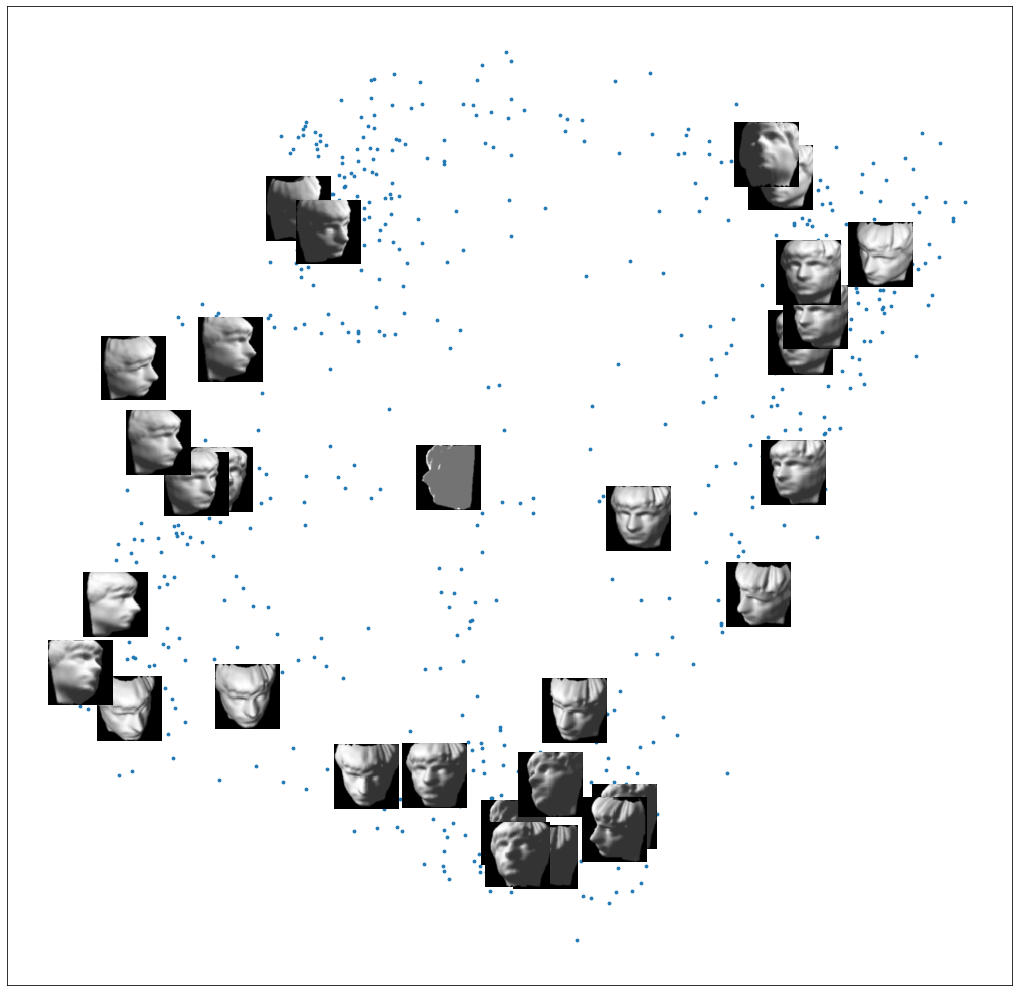
\includegraphics[totalheight=3in]{Images/Q1cgraph.png}
\end{center}
\caption{Similarity graph with Manhattan Distance}
\end{figure}

\begin{figure*}[t!]
    \centering
    \begin{subfigure}[t]{0.5\textwidth}
        \centering
        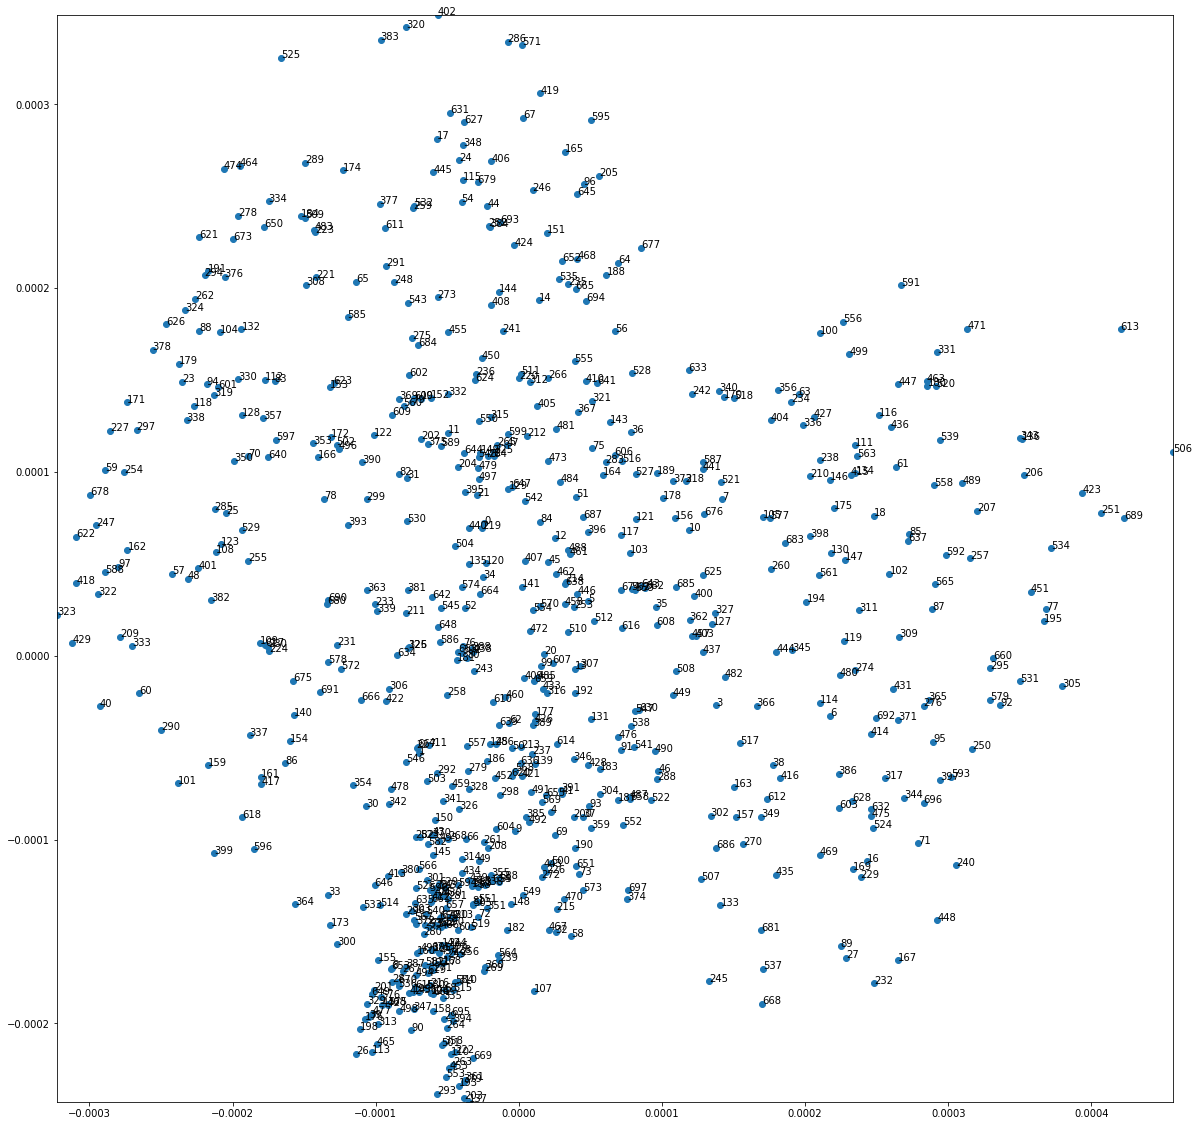
\includegraphics[height=3.1in]{Images/Q1cembedding.png}
        \caption{2D Embedding}
    \end{subfigure}%
    ~ 
    \begin{subfigure}[t]{0.5\textwidth}
        \centering
        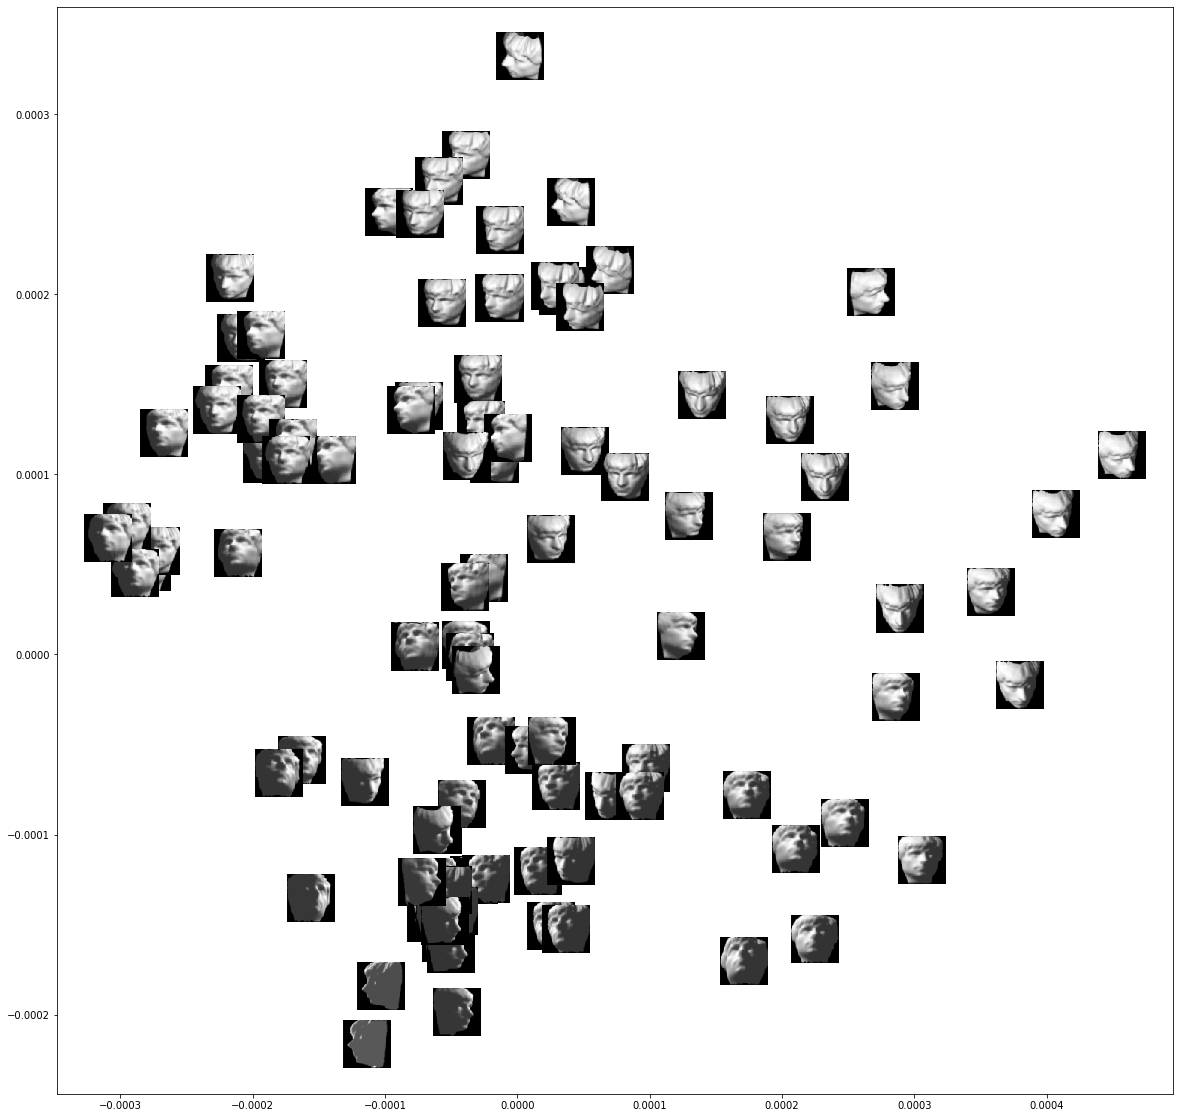
\includegraphics[height=3.1in]{Images/Q1cimages.png}
        \caption{Corresponding Images after ISOMAP}
    \end{subfigure}
    \caption{ISOMAP with Manhattan Distance}
\end{figure*}

\begin{figure}[h!]
\begin{center}
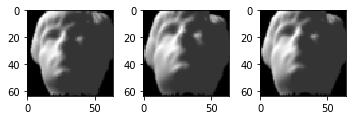
\includegraphics[totalheight=2in]{Images/Q1csimilarfaces.png}
\end{center}
\caption{Visualizing '3' close points with Manhattan Distance}
\end{figure}

\end{itemize}

\end{enumerate}

\clearpage



\subsection*{2. Density estimation: Psychological experiments. (30 points)}

 The data set \textsf{n90pol.csv} contains information on 90 university students who participated in a psychological experiment designed to look for relationships between the size of different regions of the brain and political views. The variables \textsf{amygdala} and \textsf{acc} indicate the volume of two particular brain regions known to be involved in emotions and decision-making, the amygdala and the anterior cingulate cortex; more exactly, these are residuals from the predicted volume, after adjusting for height, sex, and similar body-type variables. The variable \textsf{orientation} gives the students' locations on a five-point scale from 1 (very conservative) to 5 (very liberal).
 
  
 \begin{enumerate}
 \item[(a)] (10 points) Form 2-dimensional histogram for the pairs of variables (\textsf{amygdala}, \textsf{acc}). Decide on a suitable number of bins so you can see the shape of the distribution clearly. 
 
\begin{itemize}
\item Answer:\\
Figure 7 displays the 2 variations of the 2D histogram for the 'amygdala' and 'acc' variables.
\begin{figure*}[t!]
    \centering
    \begin{subfigure}[t]{0.5\textwidth}
        \centering
        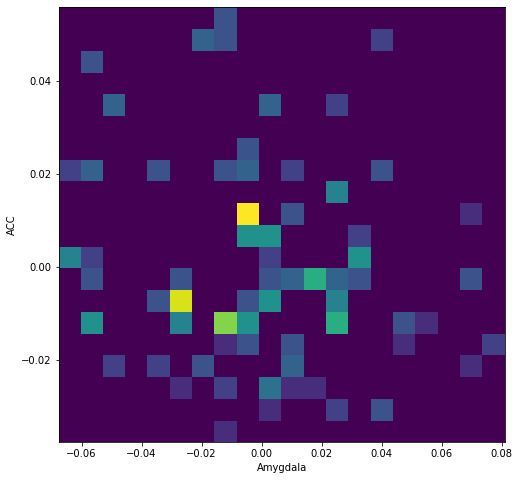
\includegraphics[height=3.1in]{Images/Q2aheatmap.png}
    \end{subfigure}%
    ~ 
    \begin{subfigure}[t]{0.5\textwidth}
        \centering
        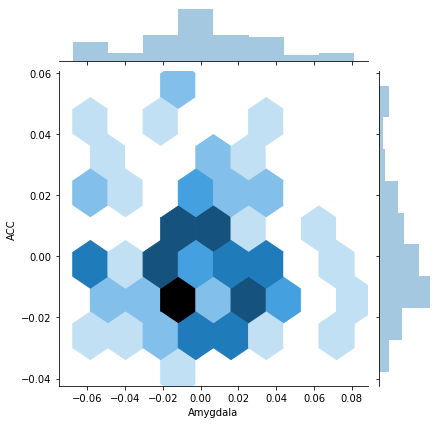
\includegraphics[height=3.1in]{Images/Q2aheatmap2.png}
    \end{subfigure}
    \caption{2D Histogram of the variables}
\end{figure*}

\end{itemize}
 
 \item[(b)] (10 points) Now implement kernel-density-estimation (KDE) to estimate the 2-dimensional with a two-dimensional density function of (\textsf{amygdala}, \textsf{acc}). Use a simple multi-dimensional Gaussian kernel, for \[x = \begin{bmatrix}x_1\\x_2\end{bmatrix}\in \mathbb R^2,\] where $x_1$ and $x_2$ are the two dimensions respectively \[K(x) = \frac{1}{\sqrt {2\pi}} e^{-\frac{(x_1^2 + x_2^2)}{2}}.\] Recall in this case, the kernel density estimator (KDE) for a density is given by
 \[
 p(x) = \frac 1 m \sum_{i=1}^m \frac 1 h
 K\left(
 \frac{x^i - x}{h}
 \right),
 \]
 where $x^i$ are two-dimensional vectors, $h >0$ is the kernel bandwidth. Set an appropriate $h$ so you can see the shape of the distribution clearly. Plot of contour plot (like the ones in slides) for your estimated density. 
\begin{itemize}
\item Answer:\\
Figure 8 displays the KDE plot of the variables.
\begin{figure}[h!]
\begin{center}
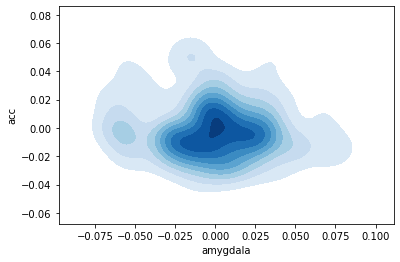
\includegraphics[totalheight=3in]{Images/Q2b.png}
\end{center}
\caption{KDE Plot}
\end{figure}

\end{itemize} 
 
 \item[(c)] (10 points) Plot the condition distribution of the volume of the \textsf{amygdala} as a function of political \textsf{orientation}: $p(\textsf{amygdala}|\textsf{orientation}=a)$, $a = 1, \ldots, 5$. Do the same for the volume of the 
 \textsf{acc}. Plot $p(\textsf{acc}|\textsf{orientation}=a)$, $a = 1, \ldots, 5$. You may either use histogram or KDE to achieve the goal. You can refer to the supplementary notes in Canvas on conditional expectation helpful.
 \end{enumerate}
 \begin{itemize}
\item Answer:\\
Figure 9 displays the conditional distributions of the respective variables. We notice that the Amygdala is more centered around 0 whereas the ACC is slightly skewed to the right, especially for orientation 2.
\begin{figure}[h!]
\begin{center}
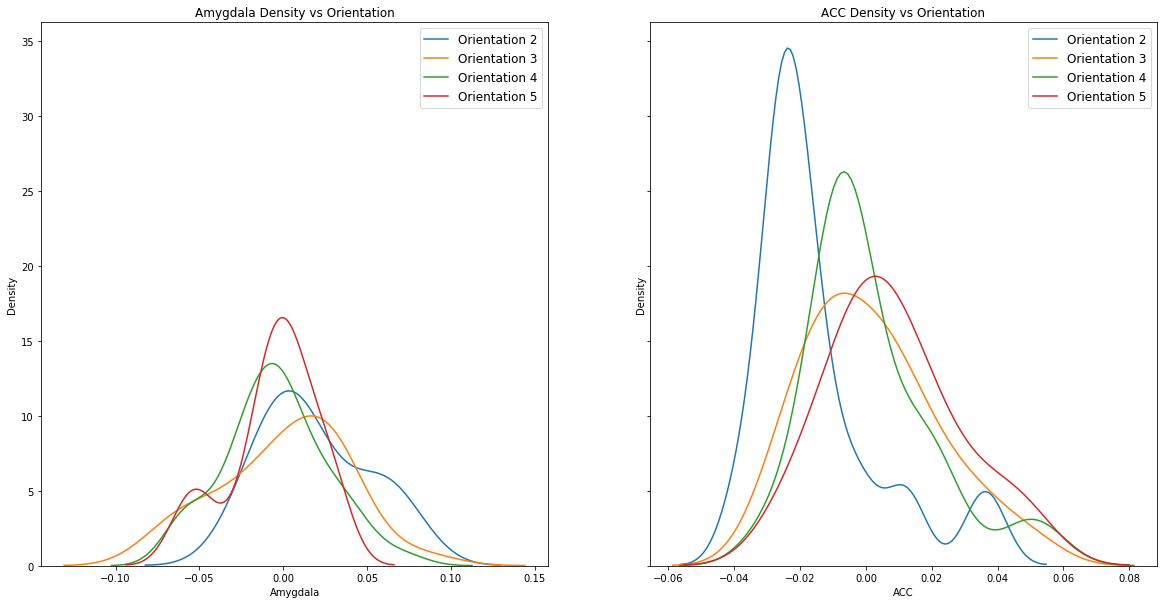
\includegraphics[totalheight=3in]{Images/Q2c.png}
\end{center}
\caption{Conditional distributions}
\end{figure}

\end{itemize} 


\clearpage

\subsection*{3. Implementing EM algorithm for MNIST dataset. (40 points)}

 Implement the EM algorithm for fitting a Gaussian mixture model for the MNIST dataset. We reduce the dataset to be only two cases, of digits ``2'' and ``6'' only. Thus, you will fit GMM with $C = 2$. Use the data file \textsf{data.mat} or \textsf{data.dat} on Canvas. True label of the data are also provided in \textsf{label.mat} and \textsf{label.dat}


The matrix \textsf{images} is of size 784-by-1990, i.e., there are totally 1990 images, and each column of the matrix corresponds to one image of size 28-by-28 pixels (the image is vectorized; the original image can be recovered by map the vector into a matrix.) 

You may find the tips in the supplementary notes useful, which explains how to evaluate the density of a multi-variate normal distribution. In this homework question, follow the low-rank approximation (with $r = 100$) to address the numerical issues.

\begin{enumerate}

\item[(a)] (5 points) Select from data one raw image of ``2'' and ``6'' and visualize them, respectively. 

 \begin{itemize}
\item Answer:\\
Figure 10 displays 2 samples images from the data.
\begin{figure}[h!]
\begin{center}
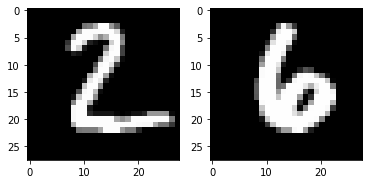
\includegraphics[totalheight=2in]{Images/Q3a.png}
\end{center}
\caption{Raw images of '2' and '6'}
\end{figure}

\end{itemize} 

\item[(b)] (10 points) Use random Gaussian vector with zero mean as random initial means, and two identity matrices $I$ as initial covariance matrices for the clusters. Plot the log-likelihood function versus the number of iterations to show your algorithm is converging.

 \begin{itemize}
\item Answer:\\
Figure 11 displays the log-likelihood vs the iteration. We notice that the algorithm converges as the number of iterations increases.
\begin{figure}[h!]
\begin{center}
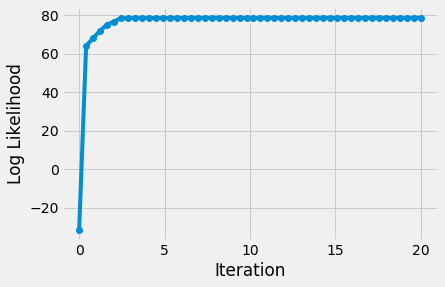
\includegraphics[totalheight=2in]{Images/Q3b.png}
\end{center}
\caption{Log Likelihood vs Iteration}
\end{figure}

\end{itemize} 
\item[(c)] (5 points points) Report, the fitting GMM model when EM has terminated in your algorithms, including the weights for each component and the mean vectors (please reformat the vectors into 28-by-28 images and show these images in your submission). Ideally, you should be able to see these means corresponds to ``average'' images.  No need to report the covariance matrices. 

\begin{itemize}
\item Answer:\\
Figure 12 shows the images after performing the GMM algorithm. The weights for '2' and '6' were 0.52 and 0.48, respectively.
\begin{figure}[h!]
\begin{center}
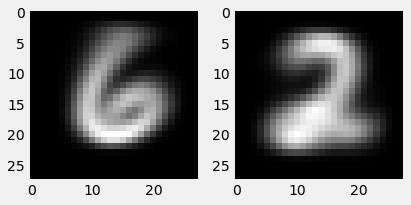
\includegraphics[totalheight=2in]{Images/Q3c.png}
\end{center}
\caption{Images after performing GMM}
\end{figure}
\end{itemize}

\item[(d)] (10 points) Use the $p_{ic}$ to infer the labels of the images, and compare with the true labels. Report the mis-classification rate for digits ``2'' and ``6'' respectively. Perform $K$-means clustering with $K=2$ (you may call a package or use the code from your previous homework). Find out the  miss classification rate for digits ``2'' and ``6'' respectively, and compare with GMM. Which one achieves the better performance?

\begin{itemize}
\item Answer:\\
Using the GMM algorithm, the misclassification rate was 0.7\%. When running the same dataset through the k-means algorithm, the misclassification rate was 6.18\%. In this case, the GMM performs much better as compared to k-means. This can be attributed to the fact that the GMM algorithm does not perform hard classifaction like k-means and instead assigns points based on probabilities.

\end{itemize}

\item[(e)] (10 points) Now first PCA to reduce the dimensionality of the data before applying to EM. We will put all ``6'' and ``2'' digits together, to project the original data into 5-dimensional vectors. Now implement EM algorithm for the projected data (with 5-dimensions). Compare the mis-classification rate of the EM algorithm using the original data (results from Part (b)-(c)), and try to explain what may cause the difference in their performance. 

\begin{itemize}
\item Answer:\\
After performing PCA and running the GMM algorithm on the new dataset, we obtain a misclassification rate of 3.37\%. The higher rate as compared to the previous part can be attributed to the fact that the PCA algorithm is reducing 784 dimensions into 5, leading to an oversimplification of the pixels and possible information loss.

\end{itemize}



\end{enumerate}


\end{document}
